% \section{Integrando las nuevas variables al dataset VarQ Curado}

En esta sección buscamos cuantificar en qué medida el esfuerzo realizado a lo largo de esta tesis mejora e impacta sobre nuestro set de datos original (VarQ). Para ello, integraremos al set VarQ Curado, que dispone de 9 features estructurales y 7,418 variantes, los features físico-químicos y genómicos obtenidos a lo largo de esta tesis.

\section{Creación del dataset Integral+VarQ Curado}
Para generar este dataset cruzamos las variantes de ambos datasets, haciendo un \textit{right-outer-join} (ver figura \ref{fig:interseccion_varq_integral}). Es decir que nos quedamos con las variantes de VarQ Curado a las que sumamos las variables del dataset Integral para aquellas variantes en la intersección de los dos conjuntos. El dataset resultante posee 73 variables, que corresponden a las 63 variables del dataset Integral sumado a las 9 variables del dataset VarQ Curado y la variable de respuesta. Este dataset posee 7,418 variantes de las cuales 5,377 (72\%) son patogénicas y 2,041 (28\%) son benignas. Las 774 variantes que no poseen variables del dataset Integral se mantuvieron en este nuevo dataset. Es por eso que en este caso la proporción de nulos para las variables genómicas es mayor que en el caso Integral, por un lado porque no se recomputaron esas variables para las variantes que no están en la intersección (774), si no que además dentro de la intersección con el dataset Integral, la cantidad de variantes sin cobertura genómica es de aproximadamente el 36\%, mientras que en el dataset Integral este valor llegaba al 20\%. Dejamos como trabajo futuro la generación de variables genómicas para las variantes de VarQ Curado no presentes en el dataset Integral.

\begin{figure}[H]
    \centering
    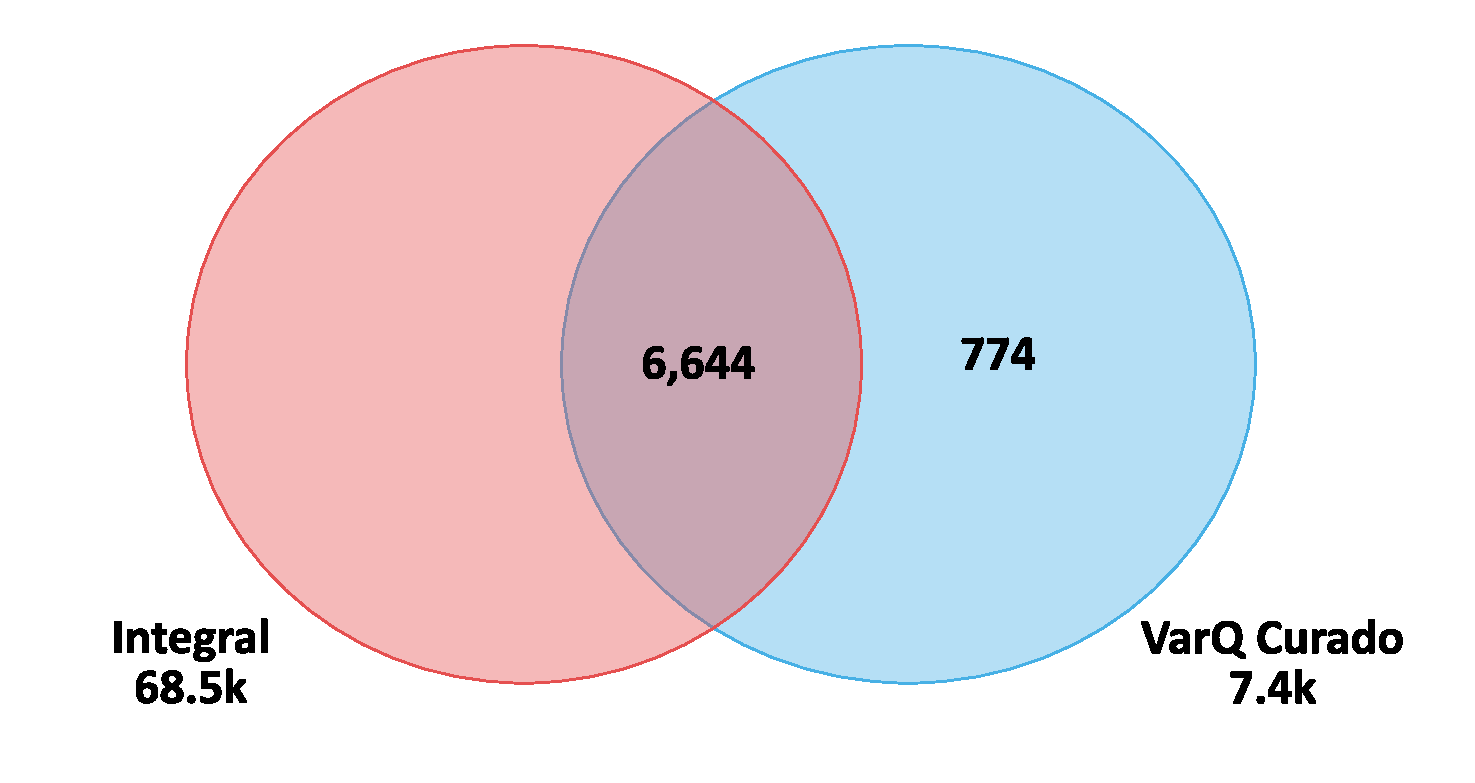
\includegraphics[scale=0.4]{documents/latex/figures/3/integral_varq/interseccion_varq_integral.pdf}
    \caption{Intersección entre los datasets Integral y VarQ Curado .}
    \label{fig:interseccion_varq_integral}
\end{figure}

\section{Generación del Modelo}
Como en los capítulos anteriores, se volvió a utilizar el Pipeline Tree para los modelos XGBoost y Random Forest. El dataset de entrenamiento posee 4,970 variantes (66\%), y el tercio restante se destinó al dataset de test. Estas variantes fueron elegidas al azar, con una semilla pseudoaleatoria para poder replicar el experimento. Este procedimiento se repitió en todos los modelos.  

\section{Resultados}
El dataset de test arrojó un AUC de 0.86 para Random Forest y 0.88 con XGBoost (ver figura \ref{fig:auc_integral_varq}). El test de DeLong \cite{DeLong} arrojó un p-valor menor a $2\mathrm{e}{-7}$, lo que nos permite aseverar que el modelo XGBoost es superior a Random Forest. Este resultado representa una mejora sensible con respecto al modelo realizado con el dataset VarQ Curado (0.74), sin superar lo obtenido por el dataset Integral (0.90 con XGBoost). Nuestra hipótesis es que esto se debe a la menor cobertura de las variables de conservación genómica. Los hiperparámetros de los modelos fueron, en el caso de Random Forest: Profundidad del árbol 7, 100 estimadores y Cantidad de variables por árbol 0.2*\textit{n} con \textit{n} la cantidad total de variables. En el caso de XGBoost, los hiperparámetros elegidos fueron:

\begin{itemize}
    \item \texttt{min\_child\_weight}: 5
    \item \texttt{gamma}: 1.5
    \item \texttt{subsample}: 1
    \item \texttt{colsample\_bytree}: 0.6
    \item \texttt{max\_depth}: 5
\end{itemize}

Considerando a la clase patogénica como clase positiva, vemos que XGBoost supera a RF en Precisión, AUC y F1-score, pero no en Recall (ver tabla \ref{tab:metrics_model_varq_integral}). Sin embargo, si tomamos a las clase benigna como positiva, el modelo XGBoost supera a RF (0.59 vs 0.53). Si bien sigue siendo un número bajo, es posible modificar el \textit{threshold} en la función de decisión en ambos modelos para obtener un Recall más alto sacrificando precisión. 

\begin{table}[H]
\centering
\begin{tabular}{|l|l|l|l|l|l|l|}
\hline
Modelo & Precisión & Recall & AUC & F1-score & $t_{fit}$ & $t_{pred}$ \\ \hline
RF  & 0.84 & 0.95 & 0.87 & 0.89 & 15.4 s & 0.07 s \\ \hline
XGBoost & 0.86 & 0.94 & 0.88 & 0.90 & 1m 20 s & 0.1 s \\ \hline
\end{tabular}

\caption{Comparación de métricas de modelos usando el dataset Integral+VarQ Curado. Las variables $t_{fit}$ y $t_{pred}$ corresponden al tiempo de entrenamiento y de predicción de todas las variantes.}
\label{tab:metrics_model_varq_integral}
\end{table}


\begin{table}[H]
\centering
\begin{tabular}{|l|l|l|l|}
\hline
             & Precision & Recall & F1-score \\ \hline
Benignas     & 0.81      & 0.53   & 0.64     \\ \hline
Patogénicas  & 0.84      & 0.95   & 0.89     \\ \hline
Promedio     & 0.83      & 0.83   & 0.82     \\ \hline
\end{tabular}
\caption{Reporte de métricas del modelo Random Forest usando el dataset Integral+VarQ Curado.}
\label{tab:metrics_integral_varq_rf}
\end{table}


\begin{table}[H]
\centering
\begin{tabular}{|l|l|l|l|}
\hline
             & Precision & Recall & F1-score \\ \hline
Benignas     & 0.80      & 0.59   & 0.68     \\ \hline
Patogénicas  & 0.86      & 0.94   & 0.90     \\ \hline
Promedio     & 0.84      & 0.85   & 0.84     \\ \hline
\end{tabular}
\caption{Reporte de métricas del modelo XGB usando el dataset Integral+VarQ Curado.}
\label{tab:metrics_integral_varq_xgb}
\end{table}

\section{Importancia de las variables}
La información proporcionada por \texttt{scikit-learn} acerca de la importancia de las variables en el modelo Random Forest están presentadas en la figura \ref{fig:importances_integral_varq}. En este ranking de las 10 variables más relevantes encontramos otra vez en primer lugar con amplia ventaja a las variables de conservación genómica, aunque también se mantiene la variación de energía y al porcentaje de SASA, que son variables pertenecientes al dataset VarQ Curado y que habían aparecido en el ranking de dicho modelo. Si consideramos la variaciones en la precisión de los modelos Random Forest y XGBoost calculados por el módulo \texttt{rfpimp} (ver figuras \ref{fig:importance_cluster_integral_varq} y \ref{fig:importance_cluster_integral_varq_xgb}), encontramos nuevamente a SNP\_DEN como una variable relevante en el modelo XGBoost, mientras que en el modelo RF aparece en el cuarto puesto con escasa diferencia de las variables con menor relevancia. VARIATION\_ENERGY y las matrices (GRANTHAM, EX, PAM250, etc.) aparecen en ambos modelos como relevantes. 


% Side by side figures 
\begin{figure}[H]
\begin{subfigure}[c]{0.50\linewidth}
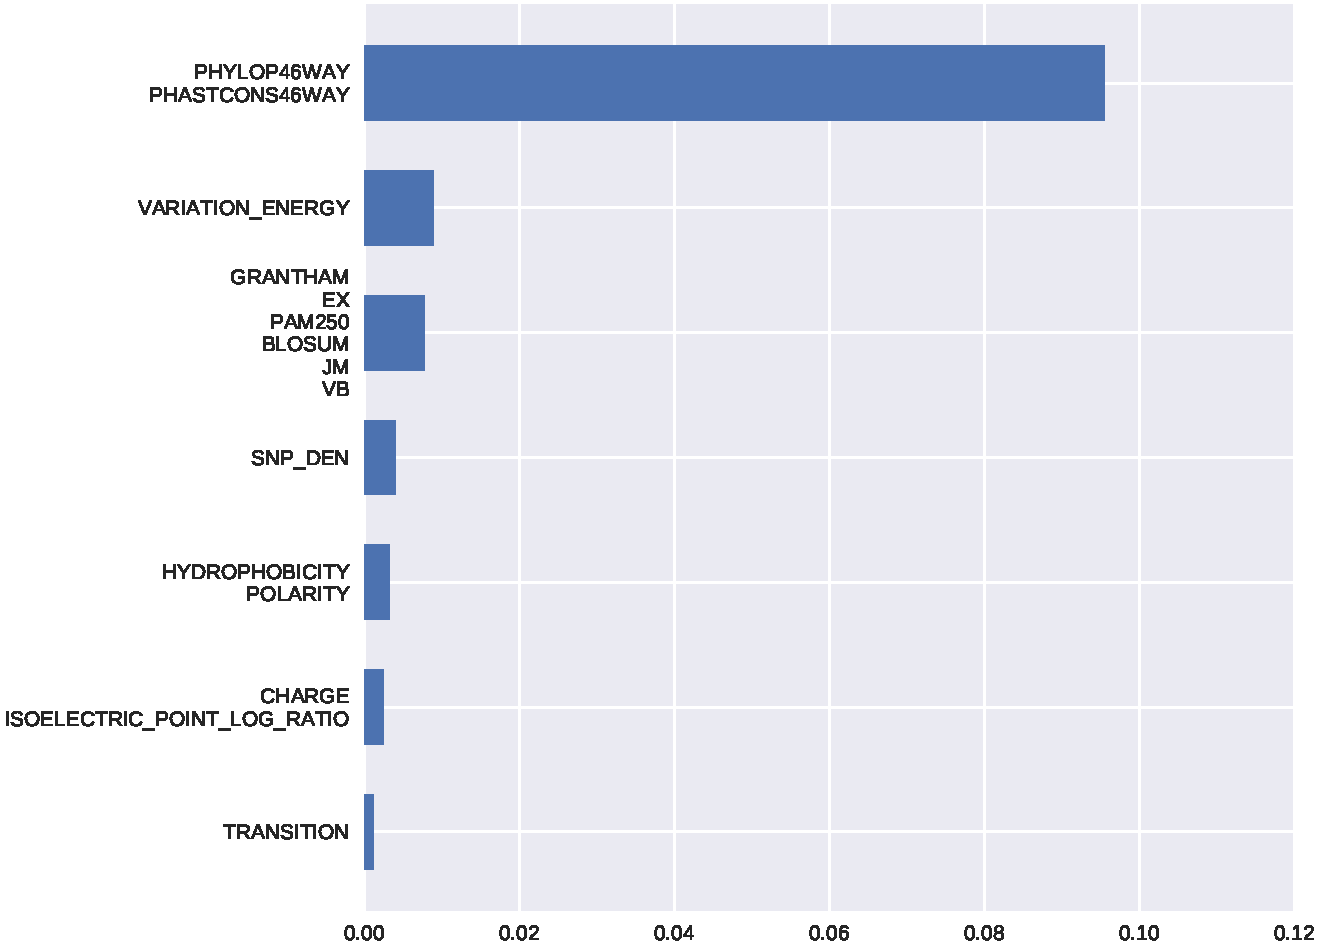
\includegraphics[width=\linewidth]{documents/latex/figures/3/integral_varq/integral_varq_importance_cluster.pdf}
\caption{Resultados del modelo usando RF.}
\label{fig:importance_cluster_integral_varq}
\end{subfigure}
% \hfill
\begin{subfigure}[c]{0.45\linewidth}
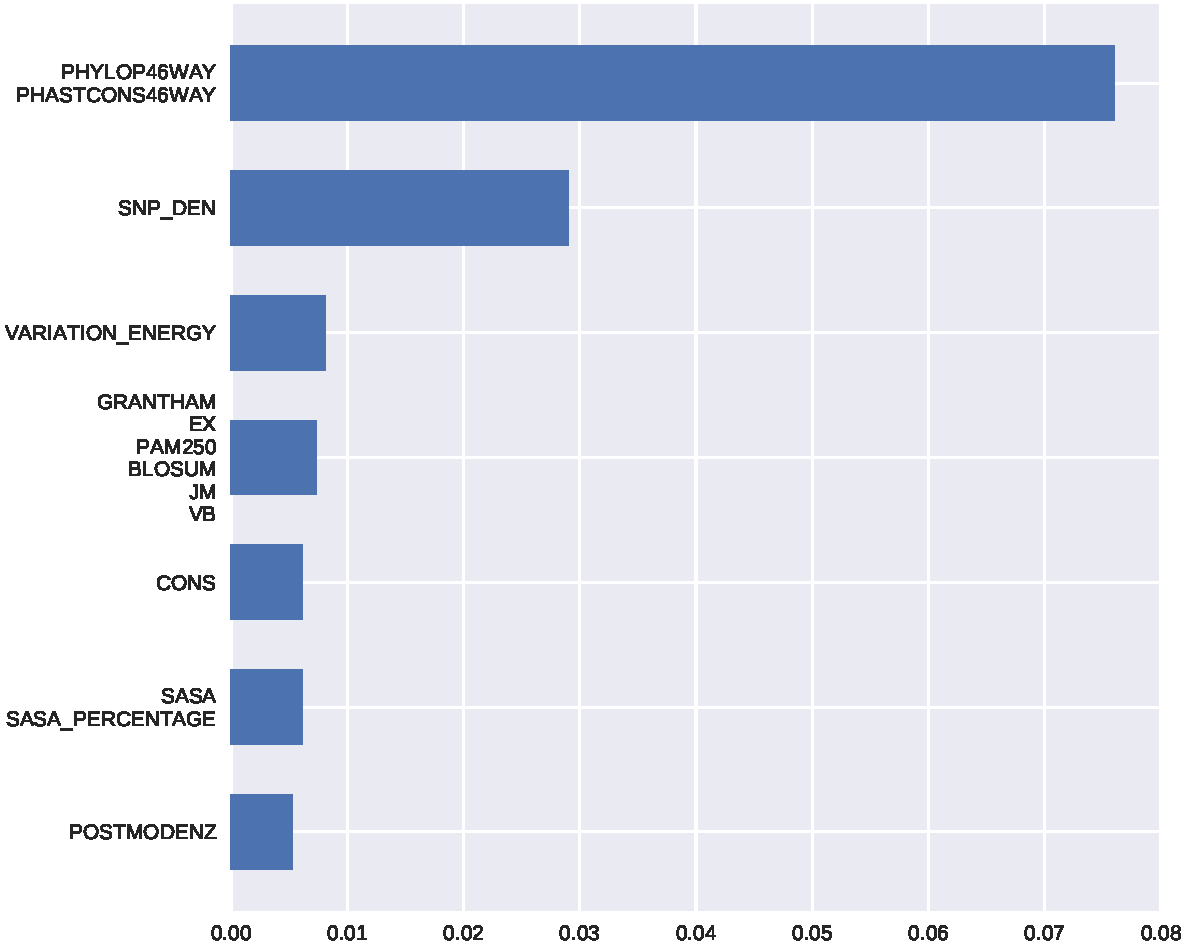
\includegraphics[width=\linewidth]{documents/latex/figures/3/integral_varq/integral_varq_importance_cluster_xgb.pdf}
\caption{Resultados del modelo usando XGB.}
\label{fig:importance_cluster_integral_varq_xgb}
\end{subfigure}%
\caption{Importancia de variables altamente correlacionadas del dataset Integral+VarQ Curado (basados en correlación de Spearman) usando permutación.}
\end{figure}



\section{Conclusión del capítulo}

La creación de un modelo combinando los datos de VarQ Curado con los del dataset Integral no superó lo obtenido por éste, aunque creemos que es posible mejorar este resultado calculando tanto las variables más importantes de VarQ (VARIATION\_ENERGY y SASA) para las variantes del dataset Integral, como las variables genómicas para las variantes del dataset VarQ Curado. 

\newpage
\begin{figure}[H]
\centering
\begin{subfigure}[b]{0.7\textwidth}
    \centering
    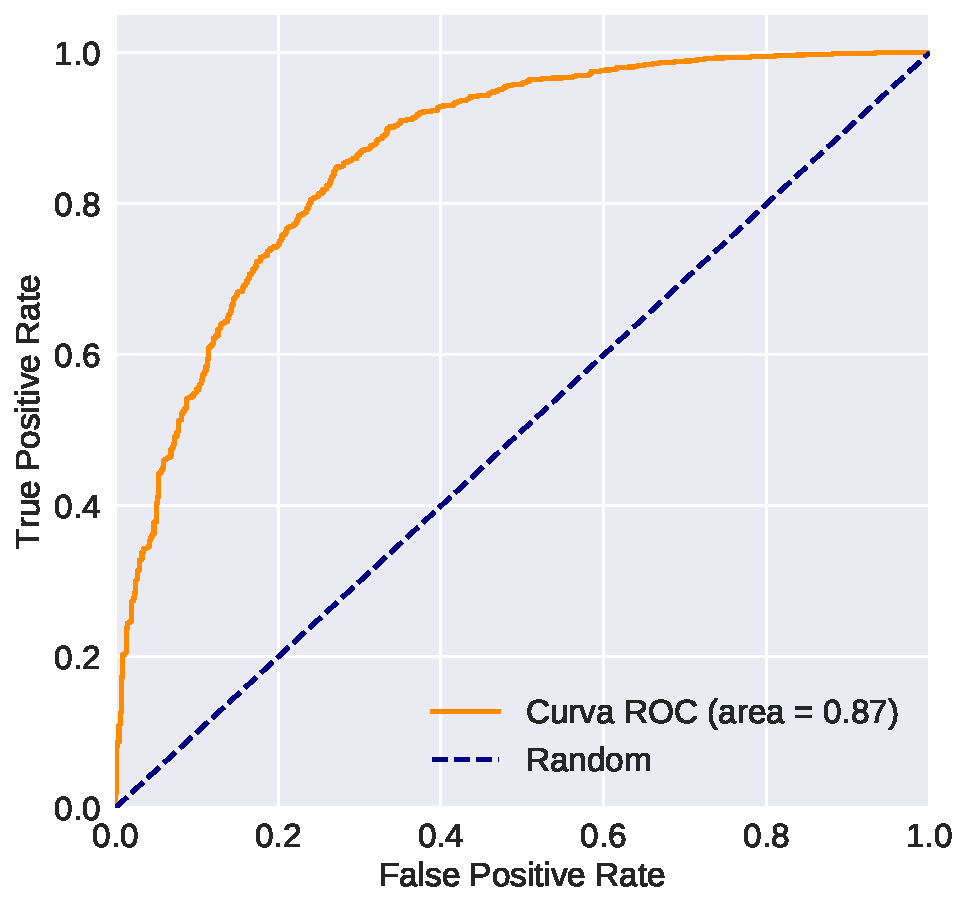
\includegraphics[width=\textwidth]{documents/latex/figures/3/integral_varq/auc_varq_integral.pdf}
    \caption{Curva AUC de los modelos Random Forest y XGBoost. La línea punteada corresponde a un predictor Random.}
    \label{fig:auc_integral_varq}
\end{subfigure}
\hfill
\hfill
\begin{subfigure}[b]{0.7\textwidth}
    \centering
    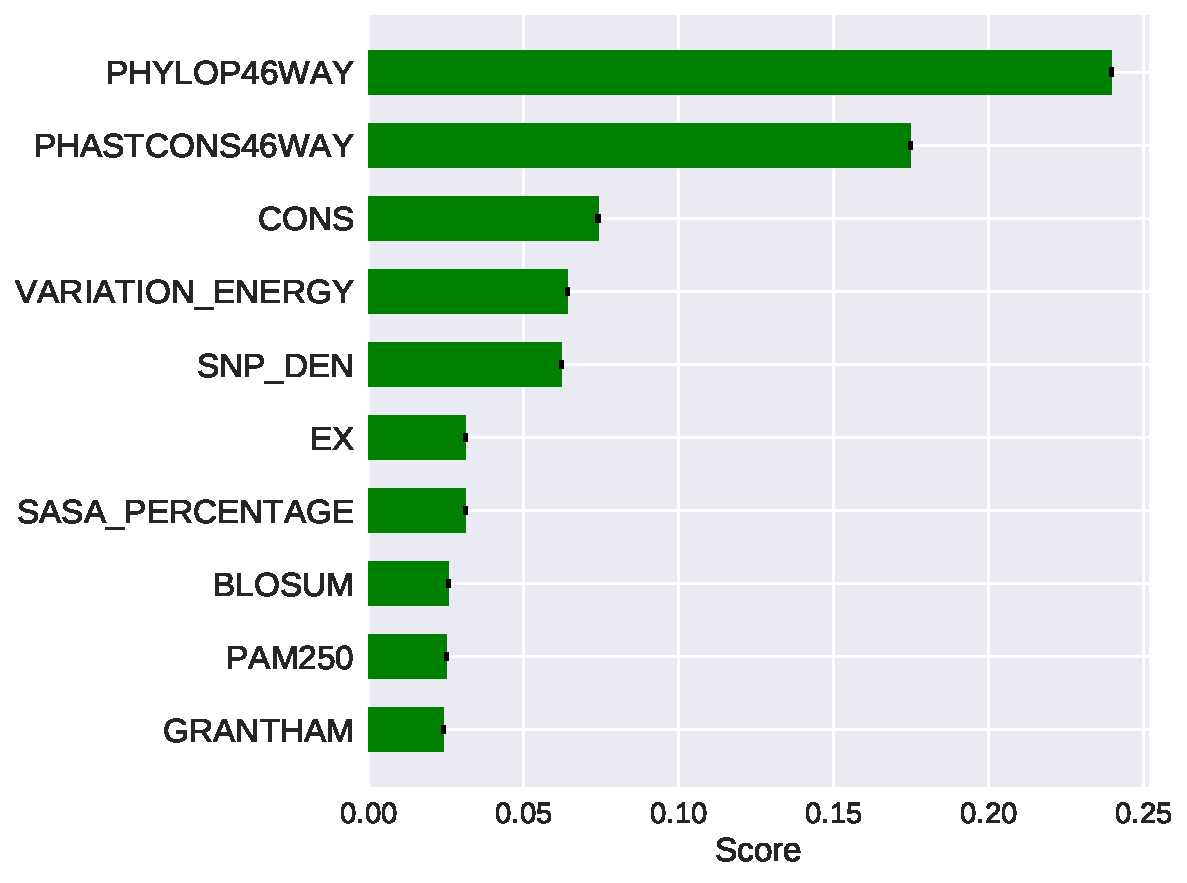
\includegraphics[width=\textwidth]{documents/latex/figures/3/integral_varq/importances_varq_integral.pdf}
    \caption{Los 10 atributos más importantes del modelo Random Forest.}
    \label{fig:importances_integral_varq}
\end{subfigure}

\caption{Curva AUC y atributos más importantes del dataset Integral+VarQ Curado.}
\end{figure}


